\section{Aufbau und Durchführung}
\label{sec:Durchführung}

Der Versuch besteht aus einer transparenten Grundplatte auf der sich ein grünes ($\lambda=\qty{532}{\nano\meter}$) und ein rotes Laserdiodenmodul ($\lambda=\qty{635}{\nano\meter}$)  befinden, welche sich im Halbkreis
verschieben lassen. Außerdem befinden sich auf der Grundplatte Metallpinne auf denen Halterungen für verschiedene optische Elemente 
platziert werden können. (siehe \autoref{fig:Abb_3} und \autoref{fig:Abb_4}!)
\begin{figure}[H]
    \centering
    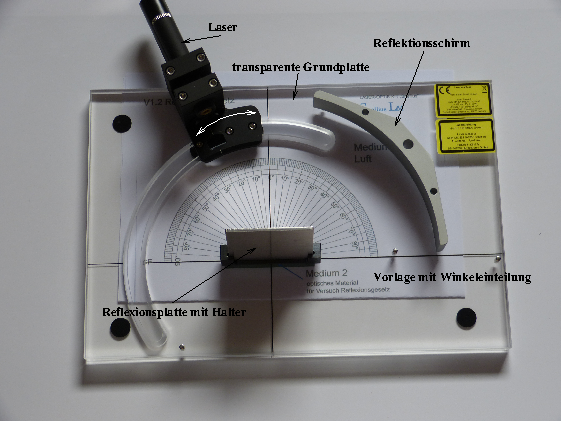
\includegraphics[width=0.5\textwidth]{build/Abb_3.pdf}
    \caption {Grundplatte mit verschiebbaren Lasermodulen \cite[1]{V400}.}
    \label{fig:Abb_3}
\end{figure}

\begin{figure}[H]
    \centering
    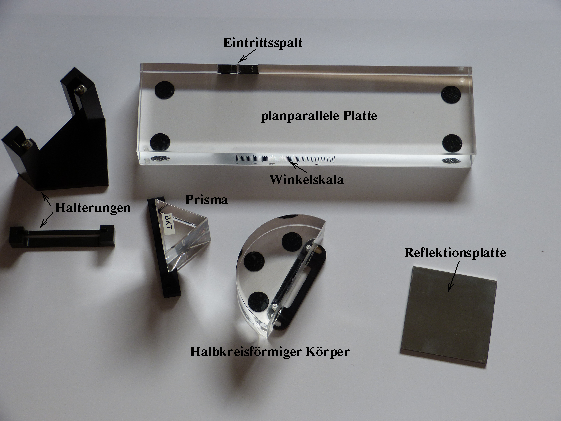
\includegraphics[width=0.5\textwidth]{build/Abb_4.pdf}
    \caption {Verschiedene optische Elemente und deren Halterungen \cite[1]{V400}.}
    \label{fig:Abb_4}
\end{figure}

Zum Schutz vor dem Laserlicht befindet sich ein Reflexionsschirm am Ende des Halbkreises, welcher beim Gebrauch beider Lasermodule
erhöht werden kann.
Außerdem gibt es verschiedene Vorlagen zum Unterlegen unter die Grundplatte, auf denen verschiedene Winkelskalen abgebildet sind.

\subsec{Reflexionsgesetz}
\label{subsec:Reflexionsgesetz_durch}

Die Vorlage A wird unter die Grundplatte gelegt. Der Spiegel wird mit der entsprechenden Halterung auf der Grundplatte platziert und
der grüne Laser eingeschaltet. Es werden $7$ verschiedene Eintrittswinkel $\alpha_1$ eingestellt und jeweils der Reflexionswinkel $\alpha_2$
abgelesen und in einer Tabelle notiert.

\subsec{Brechungsgesetz}
\label{subsec:Brechungsgesetz_durch}

Es wird wieder die Vorlage A und der grüne Laser genutzt. Die planparallele Platte wird so auf der Grundplatte platziert, dass der
Eintrittsspalt zur Winkelskala zeigt.
Es werden $7$ verschiedene Einfallswinkel $\alpha$ eingestellt und der Brechungswinkel $\beta$ jeweils an der auf der planparallelen 
Platte aufgeklebten Skala abgelesen.
Die planparallele Platte hat eine Dicke von $d=\qty{5.85}{\centi\meter}$. Anschließend wird aus den gemessenen Daten der Brechungsindex des Plexiglas und die
Lichtgeschwindigkeit im Plexiglas berechnet. Die Ergebnisse werden in einer Tabelle dargestellt.

\subsec{Planparallele Platte}
\label{subsec:Planparallel_durch}

Analog zu \autoref{subsec:Brechungsgesetz_durch} wird der Versuch aufgebaut und $5$ verschiedene Eintrittswinkel $\alpha$ eingestellt
und die Brechungswinkel $\beta$ bestimmt.
Es wird weiterhin nur der grüne Laser verwendet.
Anschließend wird der Strahlversatz mithilfe der aufgenommenen Daten berechnet.
Außerdem wird der Strahlversatz nocheinmal berechnet, diesmal jedoch nach der Bestimmunng der Brechungswinkel $\beta$ durch Verwendung
von \autoref{eqn:Brechung}. 


\subsec{Prisma}
\label{subsec:Prisma_durch}
Es werden nun der rote und der grüne Laser, sowie die Vorlage C benutzt. Zudem wird das Prisma auf der Grundplatte platziert.
Das Prisma besteht aus Kronglas und hat einen brechenden Winkel von $\gamma = \qty{60}{\degree}$.
Der Reflexionsschirm muss bei dem Versuch erhöht werden.
Es werden $5$ verschiedene Einfallswinkel $\alpha_1$ an beiden Lasern eingestellt und die Austrittswinkel $\alpha_2$ bestimmt.
Der Einfallswinkelbereich liegt zwischen $\qty{20}{degree}$ und $\qty{70}{degree}$.
Anschließend wird die Ablenkung $\delta$ berechnet.


\subsec{Beugung am Gitter}
\label{BeugungGitter_durch}

Es werden beide Laser und die Vorlage für die Beugung am Gitter benutzt.
Eine externe Winkelskala wird mithilfe von Halterungen aufgestellt und an der Vorlage ausgerichtet.
Anschließend werden $3$ verschiedene Gitter vor die Grundplatte gestellt. Die Laser werden eingeschaltet und der
Eintrittswinkel beträgt dauerhaft $\qty{0}{\degree}$. 
Für jedes Gitter werden die Beugungsmaxima der beiden Laser abgelesen und in eine Tabelle eingetragen.
Mithilfe der erfassten Daten wird die Wellenlänge der beiden Laser berechnet.
